\documentclass[11.5pt]{sig-alternate}
\usepackage[defaultlines=3,all]{nowidow}
\usepackage{hyperref}
\usepackage{tabularx}
\usepackage{graphicx}
\usepackage{blindtext}
\usepackage[utf8]{inputenc}
\usepackage[english]{babel}
\usepackage{lastpage}
\usepackage{comment}
\usepackage{dirtytalk}
\usepackage{xcolor}
\usepackage{hanging}
\usepackage{wrapfig}
\usepackage[backend=biber, style=apa]{biblatex}
\addbibresource{notation.bib}
\usepackage{authblk}
\usepackage{caption}
\usepackage{graphicx,subfigure}
\usepackage{authblk}
\usepackage{enumitem}
\usepackage[utf8]{inputenc}
\usepackage{cuted}
\usepackage{fancyhdr}
\pagestyle{fancy}
\usepackage{lipsum}
\usepackage{xurl}
\renewcommand{\headrulewidth}{0pt}
\renewcommand{\footrulewidth}{0pt}
\setlength\headheight{80.0pt}
\addtolength{\textheight}{-80.0pt}
\chead{%
  \ifcase\value{page}
  % empty test for page = 0
  \or 
\includegraphics[width=\textwidth]{headerImage.png}% page=1
  \or 
\includegraphics[width=\textwidth]{headerImage.png}% page = 2
  \or 
\includegraphics[width=\textwidth]{headerImage.png}% page = 3
  \or 
\includegraphics[width=\textwidth]{headerImage.png}% page = 4
  \or 
\includegraphics[width=\textwidth]{headerImage.png}% page = 5
  \else
  
\includegraphics[width=\textwidth]{headerImage.png}
  \fi
}
%\chead{
\includegraphics[width=\textwidth]{headerImage.png}}
\fancyfoot[LE,LO]{Perceptions of Earth Science using assistive and supportive technologies by students who are blind or visually impaired\\           
DOI: 10.14448/jsesd.13.0004}
\fancyfoot[CE,CO]{{ }}
\fancyfoot[RE,RO]{\thepage}
\pagenumbering{arabic}
\hypersetup{
    colorlinks=true,
    urlcolor=blue
}
 
\let\oldabstract\abstract
\let\oldendabstract\endabstract
\makeatletter
\renewenvironment{abstract}
{\renewenvironment{quotation}%
               {\list{}{\addtolength{\leftmargin}{1em} % change this value to add or remove length to the the default
                        \listparindent 1.5em%
                        \itemindent    \listparindent%
                        \rightmargin   \leftmargin%
                        \parsep        \z@ \@plus\p@}%
                \item\relax}%
               {\endlist}%
\oldabstract}
{\oldendabstract}
\makeatother

% Left align captions
\captionsetup{justification   = raggedright,
              singlelinecheck = false}
              
\begin{document}


\title{Perceptions of Earth Science using assistive and supportive technologies by students who are blind or visually impaired}

\author[1]{\large \color{blue} Rhea G. Miles}
\author[1]{\large \color{blue} Alana Zambone}
\author[1]{\large \color{blue}   Alex Manda}

\affil[1]{East Carolina University}

\toappear{}

\maketitle
\begin{@twocolumnfalse} 

    
\begin{abstract}
\item 
    \begin{large}
    \textit{Students with blindness or visual impairments (BVI) need to participate in scientific laboratory experiences at the K12 level to be successful in college-level science courses. These K12 level students need instruction to actively conduct science experiments and not only allow sighted students to conduct them. While it may be a challenge, with appropriate assistive and supportive technologies, students with BVI can be successful in conducting scientific investigations to address Next Generation Science Standards.  The Discoveries in Earth Science (DES) program provides engaging accommodations adaptive to the needs of elementary, middle, and high school grade students with BVI to successfully prepare for careers in STEM.}\\
    \end{large}
\end{abstract}

\end{@twocolumnfalse}

%% ABSTRACT


%% AUTHOR INFORMATION

\textbf{*Corresponding Author, Rhea G. Miles}\\ 
\href{mailto:milesr@ecu.edu}{(milesr@ecu.edu)} \\
\textit{Submitted April 15, 2021 }\\
\textit{Accepted April 04, 2022} \\
\textit{Published online October 1, 2022} \\
\textit{DOI: 10.14448/jsesd.14.0003} \\


\pagebreak
\pagebreak

\vspace{5mm}
\section*{\vspace{140mm}}
\begin{large}
\section*{Introduction}
Young students with blindness or visual impairments (BVI) have limited opportunities to participate in hands-on science activities (Supalo, 2012). Heard (2016) recommends that students with BVI participate in scientific laboratory experiences at the K12 level. K12 level students with BVI need to conduct science experiments personally and actively, otherwise, students with BVI would be at an educational disadvantage compared to their sighted peers (Supalo et al., 2007). While it may be a challenge, with appropriate accommodations such as braille labeled equipment or tools with audio assistance, young students with vision loss can be successful in conducting scientific investigations. 

A deficit of opportunities for students with BVI may stem from a dearth of knowledge of accommodations or adaptations for students with BVI or come from concern that students with BVI would be exposed to unsafe conditions or activities (Boval and Kennedy, 2018, Chapter 8). Previous work has shown that students with BVI can be successful in conducting safe scientific research and investigations with appropriate assistive technologies and modified resources (Miles Zambone, 2017). The Discoveries in Earth Science (DES) program affords accessibility to Earth science for elementary, middle, and high school students with BVI via private foundation funding and public university support.

\section*{Theoretical Framework}

There is a misconception that all students with disabilities (SWD), including those with BVI, are also cognitively impaired and this may be the case for some students in this population, but not all (Kahn et al., 2014). As reported by Joyce et al. (2020), special accommodation in communication via technological support, flexibility in scheduling activities, and flexibility in the time allotted to complete tasks can provide opportunities for SWD to learn science. Additionally, educators are responsible for facilitating as many accommodations and modifications as possible to facilitate high-quality instruction and learning (Kahn et al., 2014).

Unfortunately, many teachers are challenged to create an inclusive classroom for SWD. Most general education and science teachers are unfamiliar with teaching strategies to successfully provide instruction to SWD and seek out assistance from exceptional education teachers to best prepare and train these students with skills for employment in STEM (Griffiths et al., 2020). Kahn and Lewis (2014) found that most educators are willing to learn how to provide instruction to this marginalized group and persons with disabilities can be successfully prepared at the K12 level to pursue post-secondary degrees in STEM fields. 
	
Additional challenges include major limitations to opportunities to programs that can support students with disabilities. According to Heard (2016), there have been fewer government dollars spent to increase the percentage of students with disabilities in STEM fields than any other underrepresented population in the United States. Consequently, only 4\% of students with disabilities have earned degrees in the natural sciences (Heard, 2016). School systems are not enthusiastically incorporating STEM education into many special needs and exceptional student curricula. The implications of the limited funding and resource development for students to be prepared for STEM-related careers are a) that these students will not be interested in or fully participating in laboratory coursework, and/or b) that science teachers and teacher specialists for students with special needs do not know how to engage these students and sustain their interests and learning (Holbrook et al., 2017). Special needs students such as those with BVI have not enrolled in advanced science courses and have had limited support to pursue educational interests in scientific disciplines. 

As it states in the Next Generation Science Standards (NGSS) all students are “capable of engaging in scientific practices and constructing meaning in both science classrooms and informal settings.” (NGSS, 2013). The mantra “ Science for all” includes SWD to achieve the goals of NGSS. Furthermore, hands-on science activities assist SWD to attain and retain accurate scientific concepts (Scruggs, et al., 2017, Chapter 37). This supports the conceptual change theory which addresses changing a person from a naïve understanding of science to a more accurate one (Lynch et al., 2007). As Miller and Januszyk (2014) also report, a primary aim of NGSS is to have all students learning science and to reduce disparities in student outcomes across diverse groups, including those with disabilities. 

The NGSS emphasizes inquiry-based methods where students conduct science investigations in the natural world (Wild \& Koehler, 2017). This includes hands-on laboratory-based experiences which also support constructivist theories founded on scientific experimentation which involves students exploring problems to solve which are meaningful to them (Eliot, 2006).   A constructivist approach can promote a positive attitude and assist with developing self-efficacy which can also be effective for students with BVI (Wild \& Koehler, 2017; Hilson et al., 2016; Wild, Hilson, \& Farrand, 2013; Wild, Hilson \& Hobson, 2013; Wild \& Trundle, 2010a; Wild \& Trundle, 2010b). NGSS also promotes access to modified lab equipment and the shared expertise of science educators and teachers of the visually impaired (TVI). For example, Carabajal et al. 2017, research show that students with BVI with appropriate accommodations can successfully, comprehend and perform geoscience activities. These findings underscore the goals of the DES program. Given that there is a gap in access to science learning for students with BVI as envisioned by the NGSS, we developed the DES program to support BVI student learning and engagement. 

\section*{Discoveries in Earth Science (DES) Program}

The goal of the DES program is to provide K12 grade students with BVI the opportunity to fully engage in science. This goal aligns with outcomes from Miyauchi’s (2020) research which highlighted: 1) the ability of teachers to apply pedagogical strategies that are not highly reliant on visual instruction and demonstration 2) effective use of teaching tools, (e.g., laboratory tools with voice output); and 3) availability of external support to meet resource needs such as having a trained teacher of visually impaired (TVI) students with science knowledge or providing teachers that would devote sufficient time for the student(s) and teacher to work together. The project’s outcomes would therefore be useful for informing teachers of visually impaired students about inclusive pedagogy for this population of students.

The DES program addresses the low numbers of underrepresented groups in STEM fields by facilitating access to information and activities in Earth science. Specifically, by providing activities that are suitable for students with BVI at the K12 level, the DES program provides a unique opportunity for students in eastern North Carolina to learn Earth science in a university setting. Because one of the goals of the program is to develop the skills of students with BVI to conduct Earth science investigations, participants successfully acquire knowledge and skills to identify and characterize geologic phenomena and engage in research with minimal or no assistance from program personnel. The use of accommodations and adaptive resources by participants is critical in successfully conducting Earth science investigations.  We highlight the use of accommodations and adaptions for students with BVI in a program focusing on Earth science.

\section*{Purpose of This Study}
In this study we examine participants’, who are blind or visually impaired, perceptions and the implementation of the DES Earth science enrichment program. We pose two research questions 1) How do participants with BVI access tools to conduct Earth Science investigations? 2) How do participants who are blind or visually impaired describe their experiences in an Earth Science enrichment program?

\section*{Method}
\section*{\textit{Recruitment of DES Participants}}
Several methods were used to recruit participants for the DES program. First, directors of exceptional children’s programs in eight local school districts were contacted (through making phone calls and sending emails) to assist with the recruitment of students with BVI. Program personnel asked school district directors to contact all the parents in their databases that had identified students with BVI. Program personnel also asked the Section Chief of Sensory Support and Assistive Technology, Exceptional Children Division of the North Carolina Department of Public Instruction to recruit student participants.  Elementary, middle, and high school science coordinators from the designated school districts also assisted with recruitment. Program personnel also sent communication to the director of the state school for students with visual impairments and the regional office for people with disabilities to recruit interested students for the DES program. Other avenues of recruitment relied on personal relationships with students with BVI. For example, the director of the DES program facilitated an independent research project of a student with BVI in a prior funded program. 

A total of six students responded to the recruitment efforts, but only four students actively participated in the program. The student participants were all classified as blind or visually impaired and were served by the vision specialists at their schools. Three of the students that participated in the program were male, and one was female as presented in Table 1. Of these participants, two were black and two were Caucasian. The student participants were from grades 2 through 9.

\begin{table}[h]
\centering
\caption{\textit{Information for students that participated in the DES program.}}
\label{tab:my-table}
\resizebox{\columnwidth}{!}{%
\begin{tabular}{|l|l|l|}
\hline
Race/Ethnicity & Grade & Gender \\ \hline
Black          & 6th   & Male   \\ \hline
Caucasian      & 2nd   & Male   \\ \hline
Black          & 2nd   & Male   \\ \hline
Caucasian      & 9th   & Female \\ \hline
\end{tabular}
}
\end{table}

\section*{\textit{Description of DES Participants}}
 
Students were called participants and represented two different school districts in eastern NC. The following names are pseudonyms for the participants.  

\textit{Participant 1}. Jason was male, and in the 2nd grade. He was an honor student and a member of the talented and gifted program at his school. This participant was present for one of the three weeks during the summer session of the DES program. Jason did not continue to participate during the fall or spring semester.  During program activities, Jason relied on large print font, and a magnifying glass to see and read materials.

\textit{Participant 2}. Ben was male, African American, and legally blind. He was in the 2nd grade. He was an honor student and a member of the talented and gifted program at his school. This participant was present for most of the sessions during the three weeks of the summer DES program.  Ben also continued his participation during the fall and spring semester to work on an independent science fair project.  Ben relied on large print font, and magnification to see and read materials during program sessions. He also needed additional light, reduced glare, print on colored paper and additional time to complete his work. Moreover, he preferred to use voice output devices and an iPad to read written information and magnify words.

\textit{Participant 3}. Kevin was male, African American, and legally blind. He was in the 6th grade. His mathematics score was at grade level; however, according to his teacher assistant, his reading and comprehension was at the 1st grade level. His vision report indicates; Right 20/400 and Left 20/300 and he received assistance from the exceptional education specialist for blind and visually impaired students in the district. He wore prescription spectacles and photosensitive lenses. He received occupational and speech /language therapy as well. He also received orientation and mobility instruction but did not receive vocational rehabilitation services.

\textit{Participant 4:} Opal was a partially sighted female Caucasian participant. She had a severe case of retinopathy of prematurity.  She had mild macular dragging. Her right eye was 20/70 and her left eye was 20/100. She was an honor 9th-grade student.  She had previously completed an Earth science course in high school. 

\section*{\textit{Data Collection and Analysis}}

Numerous activities were implemented during the 3-week DES summer sessions to engage the participants in Earth Science and develop field and laboratory research skills. We intended to collect data on their use of research, adaptive technology tools through observation, records of the degree of assistance and the timeline to mastery in learning to use the tools and assistive technology: determine the program’s impact on motivation in STEM and determine curriculum content, activity experiences, and accommodations that would increase their engagement in science. Additionally, data on learning and engagement was collected through evaluation of their lab notebooks, their final projects, presentations at the end of the summer program, and their academic year activities following the summer program. 

A variety of factors limited our initial research intent, most notably the late start in funding that made it difficult to recruit a larger pool of participants and the COVID-19 pandemic, which caused all activities with K12 participants at the university to cease during the academic year and summers of 2020 and 2021.  Thus, while a variety of data was collected, researchers focused on participants’ engagement and as a pilot study to refine DES summer and academic year curricula activities for research questions and design.  Therefore, the analysis focused on student engagement after participation in activities implemented during the 3-week DES summer session.  Each participant at the end of the day was asked “What is your favorite “thing” you did today?” Participant responses were audio recorded and transcribed.  All data were coded and entered into Microsoft Excel spreadsheet by the researchers. 

Spradley’s (1980) developmental research sequence was used to guide data analysis of the participant-observer field notes and the open-ended questions asked of participants. This analysis led to establishing categories. A classification scheme was developed by the researchers using Tesch’s (1990) organizational system where observations and responses were broken down into units and segments containing one complete idea pertinent to the research questions. Researchers reviewed the field notes collected by a passive participant- observer who only engaged when one of the participants spoke directly to him or her or asked for assistance in using a tool such as the Vernier salinity probe, and an active participant-observer who facilitated students’ participation in the science activities and transcriptions of the four participants’ responses. Neutrality was maintained during our inter-rater analysis as data was examined and categorized on emerging themes (Patton, 2002). As we were concerned with increasing participants’ engagement in the science and their knowledge and skills in using the tools and concepts to conduct scientific study, we noted that themes emerged related to the facility with tools and procedures, interest in science concepts and activities, future opportunities to pursue science careers, and scientific methods and approaches. Data indicating these themes included decreasing time to initiation of an activity, changes to the types of assistance they requested, participants’ questions, comments, and discussions of their findings and their feedback on the day and the activities. For example, the time it took the participants to set up and begin to engage in an activity decreased and the request for assistance also decreased and began to focus on supports for accessing information visually or more in-depth information. Discussions amongst them shifted over time from when lunch would be served or interest in what the adults and other participants were doing to what they were finding in their science activities. Conversations about their school and community experiences began to shift to discussions about what they wanted to do for their science projects during the academic year between summer program sessions.

Participant responses were categorized as related to either assistive or supportive technologies. Assistive technologies were defined as those resources ( i.e., tools and equipment ) that the students could use independently, with very little assistance, and were designed for students with BVI. Supportive technologies were defined as resources (i.e., tools and equipment) that require instructor assistance or are used by seeing students as is. Refer to Appendices A and B for participant responses. Responses categorized as assistive technologies were the Talking LabQuest Talk 2 Probes and braille protractors and responses categorized as supportive technologies included topographic maps, fossil identification, water level meter, water collection devices at site, mineral identification, rock identification, and the augmented reality sandbox. Refer to Appendix C for information about materials, name of place, and link to purchase memorable assistive and supportive technologies.
\section*{DES Project Goals: Adaptations and Accommodations}

Successful adaptations and accommodations of the memorable experiences for the DES participants while using assistive and supportive technologies are described below. Descriptions of participants conducting investigations using the Water Level Meter, Water Collection Device, LabQuest Talk 2 and Probes, Rock Identification Kit, Mineral Identification Kit, Fossil Identification Kit, Topographic Map, and Augmented Reality Sand Box are provided.  Some pictures of participants using the devices and a sample of completed data sheets are also shown in Figures 1, 2 ,3, 4, 5, 6, 7, 8 and 9.

\section*{\textit{Water Level Meter}}

A Water Level Meter is an instrument that is used to measure the depth to the water table in a groundwater well. The Water Level Meter has a measuring tape set on a stand-alone reel with an on/off switch, brake and carry handle. On the tape there are permanently embossed black graduations that are used to show the depth to the water level. The meter is equipped with a sounder that makes a beeping noise when the sensor at the end of the tape touches water.

\section*{\textit{Adaptations/Accommodations}}

The participant had to practice holding the measuring tape between the appropriate fingers and then loosen fingers to drop the line into the groundwater well.  When a sound was heard to indicate that the tape measure had reached the water in the well, the participant would pinch the tape measure to mark the depth of the water table as illustrated in Figure 1.
\\
\begin{figure}[htp] 
    \centering
    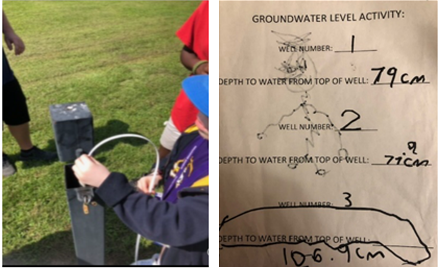
\includegraphics[width=8cm]{figure1.png}
    \caption{Participant using water level meter to make  groundwater level well measurement and sample recorded data }
    \label{hands-on Bohr model using Styrofoam}
\end{figure}


Next, the participant would pull the measuring tape out of the well and ask for assistance of another DES participant to grab the other end while also holding on to the tape measure.  Since the numbers and units on the tape measure on the water level meter were very small and difficult to view, the DES participant would use a talking tape measure to determine the depth of water in the well. The talking tape measure was then lined up next to the water level meter, and the measurement was provided through audio sound on the device. The participant then had to record the well number and depth of the water from the top of the well on a “Groundwater Level Activity” sheet presented in Figure 1. A participant also had the option to save the data in the talking tape measure, however each participant was required to record information on a data sheet. Participants recorded data on a sheet where information was written using 20-point font. DES program personnel provided additional assistance by pointing to where a participant would fill in information on the data sheet.  
\newpage
\section*{Water Sampler}

In addition to collecting water in groundwater wells, participants also collected water from a stream and river. The DES participants used a Water Sampler, which is a sample bottle attached to a long yellow pole, to collect water samples as shown in Figure 2.
\\
\begin{figure}[h] 
    \centering
    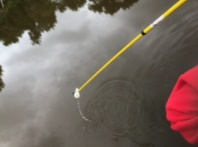
\includegraphics[width=\columnwidth]{figure2.png}
    \caption{Using water sampler device }
    \label{hands-on Bohr model using Styrofoam}
\end{figure}

\section*{\textit{LabQuest Talk 2 and Probes}}
 
The DES participants analyzed water samples collected in the field using Vernier LabQuest Talk 2  device and associated probes to conduct temperature, salinity, pH, and conductivity measurements using the text to talk speaking feature. 

\section*{\textit{Adaptation/Accommodation}}

With minimum assistance from staff the DES participants were guided to use the probe and glassware to familiarize themselves with collecting and analyzing data. The DES participants learned to select and use the appropriate probes for temperature, salinity, pH, and conductivity measurements.  After taking the measurements, the participants listened to the readings before recording data on their data sheet as seen in Figure 3.
{\begin{figure}[htp] 
    \centering
    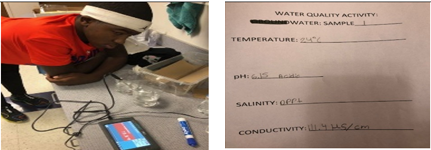
\includegraphics[width=8.5cm]{figure3.png}
    \caption{Participant listening to Lab Probe Talk 2 Device and recorded data }
    \label{Lab Probe Talk 2 Device and recorded data }
\end{figure}
}

\section*{\textit{Rock identification}}

DES participants were first introduced to rocks through a Rock Identification Kit. The participants were given the name of a sedimentary, metamorphic, or igneous rock to write on their data sheet.  Participants were instructed to mark on the data sheet if a given sedimentary rock color was light or dark and the texture was fine or course.  Each participant also added a few drops of dilute acid to hear whether the sedimentary rock fizzed and formed bubbles to test for carbonate minerals. The color, texture, and presence of carbonates for both the igneous and metamorphic rocks were determined similarly to the sedimentary rocks. However, for the metamorphic rocks the participants were instructed to determine whether there was foliation or no foliation and banding or no banding. They marked their data sheets accordingly.  Additionally, for igneous rocks the participants were to mark whether the igneous rocks were glassy or not glassy and given instructions on how to determine, low, intermediate, or high density. Participants were also given a metamorphic rock identifications flow chart to read further about other characteristics and information of given identified rocks. Furthermore, for igneous rocks, participants were informed about where the rock was found such as in a volcano or inside the Earth. The participants were given unknown rock samples and were to write down and describe characteristics to determine the identity of the rock based on given written information.  

\section*{\textit{Adaptation/Accommodations}}
  
As shown in Figure 4.a, all participants used magnifiers to better identify a rock.  Additionally, in lieu of visual prompts to help participants identify the rocks and complete their data sheets as presented in Figures 4.a and 4.b, students were prompted tactually to guide their hands in exploring rocks and to direct them in recording their data in the appropriate section on their data sheets. Participants marked and recorded data in boxes which were a different color from the background paper.

\begin{figure}[h]
   \renewcommand{\thefigure}{4a}
        \centering
        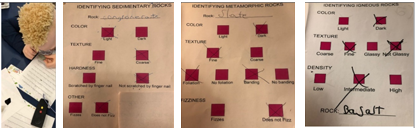
\includegraphics[width=8cm]{figure4_1.png}
        \caption{Participant completed data sheet for \\identifying sedimentary, metamorphic, and igneous rocks }
        \label{Participant completed data sheet }
    \end{figure}

    \begin{figure}[h]
      \renewcommand{\thefigure}{4b}
        \centering
        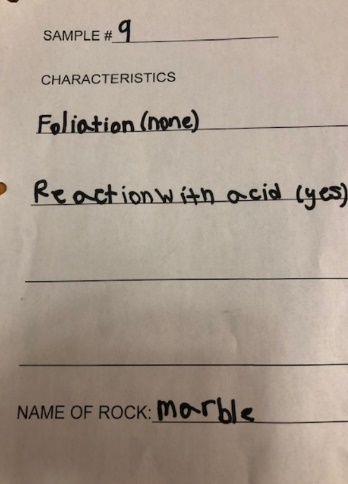
\includegraphics[width=8cm]{figure4_2.png}
        \caption{Participant rock identification of unknown \\rock samples }
        \label{ Participant rock identification of unknown rock samples}
\end{figure}
\newpage
\section*{\textit{Mineral Identification }}
Participants learned from DES personnel how to determine the following information for mineral identification which included: color streak, cleavage, cleavage plane, luster, hardness, reacts with acid (fizzes) and magnetism. 

\section*{\textit{Adaptation/Accommodations}}
 Color streak was determined using a Colorino device that identifies colors. This talking device let the user know the color of the sample. A traditional streak on a plate or paper was not done since the streak was too small for the participants to “see” and Colorino would not work properly on less than a 5 cm by 5 cm area surface. Thus, the Colorino probe was placed directly onto the mineral and the color would be said aloud by this audible device. The participants would mark the appropriate box in the data sheet to identify a given mineral. All participants were able to mark a box to identify a mineral if the box was a different color from the background paper.  Participants marked and recorded data in boxes which were a different color from the background paper. Refer to Figure 5 for completed participant data sheet.
\begin{figure}[htp] 
  \renewcommand{\thefigure}{5}
    \centering
    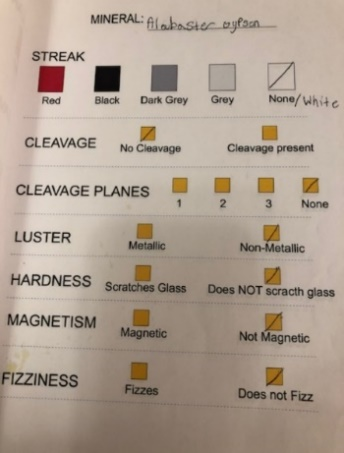
\includegraphics[width=8 cm]{figure5.png}
    \caption{Participant completed mineral data sheet.}
    \label{Participant completed mineral data sheet. }
\end{figure}

\section*{\textit{Braille Protractor}}
 
A braille protractor with a pivoting wand was used to measure interface angles of various minerals as shown in Figure 6. 

\begin{figure}[htp] 
  \renewcommand{\thefigure}{6}
    \centering
    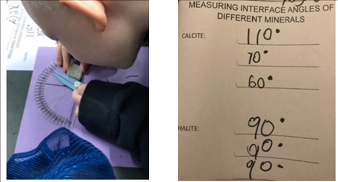
\includegraphics[width=8 cm]{figure6.png}
    \caption{Participant using braille protractor and completed data  }
    \label{ participant using braille protractor and completed data  }
\end{figure}

The American Printing House (APH) braille protractor has large print and raised dots every 5 degrees for the 180-degree protractor. Since the lines on the braille protractor were also bold and the numbers were 18-point font, even participants who could not read braille could use the device. 
\section*{\textit{Adaptation/Accommodations}}
The participants were trained to use the instrument on models with predefined angles by helping them locate the pivoting wand and getting acquainted with the units of measurement. Once students had sufficient practice with the instrument, they progressed to measuring angles of minerals themselves. 
\section*{\textit{Fossil Identification}}Fossil Identification
n Each DES participant was asked to draw and describe a given fossil on a given data sheet. 

\section*{\textit{Adaptation/Accommodations}}

 Fossils from a Fossil kit were made into three dimensional (3D) models which were enlarged by 3 times their original size using a MakerBot 3D printer.  Additionally, two of the four participants used a document camera to further magnify the fossils to complete the data sheets as shown in Figure 7.
{\begin{figure}[htp] 
  \renewcommand{\thefigure}{7}
    \centering
    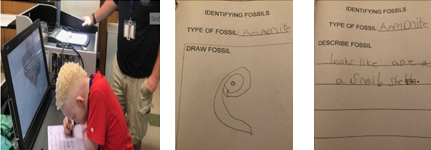
\includegraphics[width=7.75cm]{figure7.png}
    \caption{Participant recording characteristics of fossils and sample completed data sheets for recording information about fossils }
    \label{ Participant recording characteristics of fossils and sample completed data sheets for recording information about fossils }
\end{figure}
}


\section*{\textit{Topographic Maps}}
DES participants also learned the basic skills for reading topographic maps which included determining latitude and longitude using raised relief maps as shown in Figure 8. The participants also used the maps to determine the cardinal directions on a map: east, west, north, and south.  

{\begin{figure}[htp] 
  \renewcommand{\thefigure}{8}
    \centering
    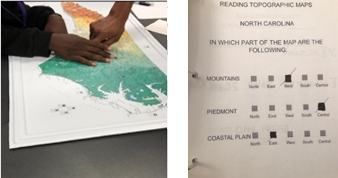
\includegraphics[width=7.5cm]{figure8.png}
    \caption{Participant reading topographic raised relief map of North Carolina and sample completed data sheet }
    \label{ Participant reading topographic raised relief map of North Carolina and sample completed data sheet  }
\end{figure}
}
\section*{\textit{Adaptation/Accommodations}}
Large braille stickers were placed on the topographic maps to indicate map direction  (i.e., north, south, east, and west).  Each participant was able to learn the braille symbols for East, North, West, and South.  Stickers with a font size of 20 were also placed on these maps to aide participants with determining latitude and longitude. The participants would touch the topographic maps of North Carolina to determine the location of the piedmont, coastal and mountain regions.

\section*{\textit{Augmented Reality Sandbox}}
An Augmented Reality Sandbox consisted of a table filled with sand, a scanner, and a projector. The scanner detected the height and placement of the sand in the basin, calculated the appropriate projection, and transmitted the information to the projector, which then projected topographic lines and colors onto the corresponding sand below. The participants were asked to use their hands to make models of landforms such as Mt. St Helens, Mt. Rainier, and the Grand Canyon in the augmented reality sandbox.  
\newpage
\section*{\textit{Adaptation/Accommodations}}
 DES participants would wrap their hands around a 3-D model of the landform of interest. After a few minutes feeling the features of the 3D model, the participants would then recreate the landform in the augmented reality sandbox as seen in Figure 9.  

\begin{figure}[h] 
  \renewcommand{\thefigure}{9}
    \centering
    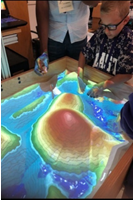
\includegraphics[width=\columnwidth]{figure9.png}
    \caption{Participant using augmented reality sandbox }
    \label{ Participant using augmented reality sandbox }
\end{figure}
 
\section*{\textit{Other Summer Activities}}
Interestingly, there were several other activities that did or did not require assistive or supportive devices such as talking calculators; however, the participants did not remember them. For example, DES participants and staff traveled to a fossil museum where an accommodation included having the names of the fossils written in braille to allow DES participants to identify them.  The participants were also given Styrofoam and plastic models to demonstrate the orientation of layers in rocks and faulting resulting from deformation of rock units. Additionally, participants used playdough to better understand the concepts of superposition and foliation. Furthermore, participants used fault blocks models, physical models, sandpaper, aluminum foil, and braille stickers to distinguish the three major fault types (reverse, normal, and strike slip) and recognize different types of folds (synform and antiform).  They appeared to have fun and enjoyed their DES experiences but did not mention all of their experiences.

\section*{\textit{Safety}}
The majority of DES investigations did not require the use of gloves or safety goggles. Only one investigation when DES participants were using dilute acid to test for the presence of carbonates required the use of safety goggles and gloves. DES investigations during the summer and academic year were designed to require minimum protection for eyes, hands, or body for the elementary, middle and high school participants. The participants used personal protective equipment where appropriate. 

\section*{\textit{Safety Academic Year Sessions}}
After participating in the 3-week summer program, all four of the participants were encouraged to conduct individual investigations during the academic year. Three of the four participants designed and developed individual science fair projects during the academic year. They used assistive or supportive technologies to conduct their individual projects. Of the four participants, only two, Ben and Opal developed projects that were presented at the regional science fair in the state.  

\section*{\textit{Ben’s Project}} 
Ben wanted to investigate what type of rocks were where he lived for his Science Fair project as shown in Figure 10.  Ben’s investigation focused on determining whether the rocks in the nearby park were metamorphic. He used several techniques to identify rocks and the minerals in the rocks. 

\begin{figure}[htp] 
  \renewcommand{\thefigure}{10}
    \centering
    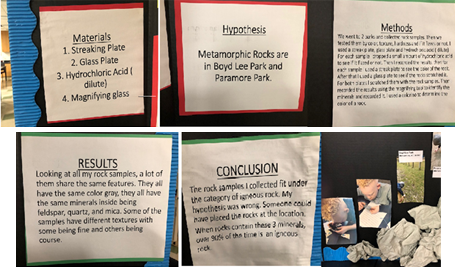
\includegraphics[width=\columnwidth]{figure10.png}
    \caption{Ben’s  final science fair project }
    \label{ Ben’s  final science fair project }
\end{figure}

\section*{\textit{Adaptation/Accommodations}}
 Ben went to two nearby parks and searched for rocks on the ground. When he found a rock, he applied the process of rock identification described above to try to identify the rock.
 \newpage
\section*{\textit{Opal’s Project}} 
For Opal’s science fair project as seen in Figure 11, Opal focused on collecting local stream water and comparing it with filtered water (bottle and tap water) to determine whether the water samples were in the appropriate ranges for safe drinking water. She used a LabQuest Talk 2  and probes to measure the salinity, conductivity, temperature, and pH of the water samples.  In addition, she used the AM 12 LaMotte: The TESTABS Water Investigation Kit to measure alkalinity, dissolved oxygen, ammonia, iron, nitrates, chloride, and phosphate levels in the water samples. These kits included tablets that changed color depending on the properties of water samples being analyzed.  

\begin{figure}[h] 
  \renewcommand{\thefigure}{11}
    \centering
    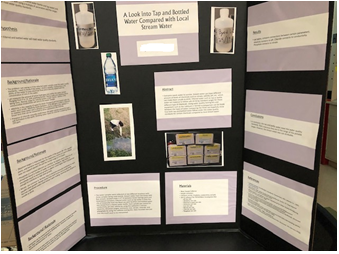
\includegraphics[width=\columnwidth]{figure11.png}
    \caption{Opal’s final science fair project}
    \label{Opal’s final science fair project}
\end{figure}

\section*{\textit{Adaptation/Accommodations}} 
To complete her investigation the test tabs were handed to Opal to use. After designated tablets were added, a talking timer was set to indicate when to observe the color changes of the water samples.  Any changes to color were verbalized to Opal, after which she was able to record information in her data table. Opal earned first place in the regional competition. Unfortunately, the state science and engineering fair was canceled due to the COVID-19 pandemic.

\section*{\textit{Challenges of DES Program}}
Additionally, participants did respond favorably to many of the assistive and supportive technologies, but naturally, there were some challenges faced by participants of the DES program. Measuring with the braille graduated cylinders to determine volume was not as user-friendly as was expected as only one participant could read braille. Additionally, the precision of the audible instruments to measure volume could not measure small changes in the water displacement volumes of small rocks or minerals. Challenges faced in the program were related to the inadequacies of the devices and tools for students with BVI used in the activities rather than the participant unfamiliarity with the tools.

\section*{Discussion and Conclusion}

As noted above, the DES program’s summer and academic year activities served to provide elementary, middle and high school grade students with BVI the opportunity to fully engage in science. DES addressed the research questions and design to provide information about access to tools to conduct Earth Science investigations and descriptions of their experiences in an Earth Science enrichment program. The participants of the DES program accessed tools to conduct Earth science investigations using assistive and supportive technologies (see to Figures 1-9).  The DES program focused on approaches to meet the needs of students with BVI by (a) highlighting new technologies and (b), refining and revising accommodations to best suit the unique needs of participants. DES personnel were able to provide one-on-one assistance to participants during the 3-week summer program and provide direct individualized assistance during the monthly sessions in the academic year. 

Even though this study is limited to the small population who participated in the DES program, findings are applicable to other students with BVI and formal classroom use. The DES program provided participants with BVI the opportunity to fully engage in science by using assistive and supportive technologies to conduct and collect data themselves as seen in Figures 1 through 9.  After participation in a science fair, some participants developed communication skills and a desire to want to conduct scientific investigations.  This program’s outcomes also inform classroom teachers about inclusive pedagogy for this population.  Assistive and supportive technologies are available for students with BVI for classroom teachers to include in their implementation of strategies in science instruction. The results from the engagement of a small population of students in the DES program show promise for a larger participant population where additional metrics for attitudes and learning outcomes might inform a broader population of students with BVI. The DES program aligns with Miyauchi’s (2020) research which focuses on a) identifying effective instructional approaches and practices and b) providing the participants with supportive and assistive technology. 

Unfortunately, not all students with BVI have access to technologies and teacher instruction as previously described for the DES program.  When students with visual impairments are physically in the science education environment, they often do not participate in science experiments (Koehler \& Wild, 2019; Miles \& Zambone, 2017)  Although students with visual impairment are capable of studying all academic subjects like their peers, they are known to be excluded from participating in all subject-related activities, particularly in mathematics, science, physical education (Kahn et al., 2014) and advanced-placement science classes (Koehler \& Wild, 2019). Moreover, “students with visual impairment choose courses based not on their ability and interests, but on accessibility” (Miyauchi, 2020, p.2).  In our study, we found that the DES program provided greater accessibility to science through the activities implemented with assistive and supportive technologies (see Figures 1-9).

Furthermore, as discussed in Miyauchi’s work:  “ the level of accessibility of the course depends heavily on the subject teacher’s knowledge and willingness” to provide instruction to students with BVI (Miyauchi,2020,  p. 2 ). Miyauchi’s research (2020) accounts for this limited access as related to teachers having little or no: 1) pedagogical strategies other than a generic set that is highly reliant on visual instruction and demonstration 2) tools, particularly assistive technology such as laboratory tools with voice output; and 3) external support such as a trained TVI with science knowledge or sufficient time for the student and teacher to work together.  The DES program further provided possibilities for students to work together with teachers. Eventually, DES participants gained confidence and knowledge to conduct scientific experiments using the assistive and supportive resources to complete scientific projects.  As advocated by Edelson et al. (2021) and Griffiths et al. (2020) the outcomes of the DES program addressed the goals of the NGSS by making learning about science more meaningful and assisting with better preparing students with blind or visual impairments for the STEM workforce.  

\include{} 
\section*{References}
\par 

\leftskip 0.25in
\parindent -0.25in 
%%%

Boval, J. \& Kennedy, S. (2018) Laboratory Safety for All: Accommodating students with disabilities in chemistry teaching laboratories. In: Sweet, E., Gower, W.S. \& Heltzel, C. E. \textit{Accessibility in the Laboratory}. Washington, D.C.: American Chemical Society. doi: 10.1021/bk-2018-1272.ch008

Carabajal, I.G., Marshall, A.M., \&  Atchison C.L., (2017). A Synthesis of Instructional Strategies in Geoscience Education Literature That Address Barriers to Inclusion for Students With Disabilities. \textit{Journal of Geoscience Education, 65}(4), 531-541. doi: 10.5408/16-211.1

Edelson, D.C., Reiser, B.J. , McNeill, K.L., Mohan, A., Novak, N., Mohan, L. A. Affolter, A., McGill, T. A. W., Bracey, Z.E.B., Noll, J.D., Kowalski, S.M., Novak, D., Lo, A.S.,  Landel, C., Krumm, A., Penuel, W., Van Horne, K., González-Howard, M., \& Suárez, E. (2021). Developing Research-Based Instructional Materials to Support Large-Scale Transformation of Science Teaching and Learning: The Approach of the OpenSciEd Middle School Program. \textit{Journal of Science Teacher Education}, 32(7), 780-804, \\doi: 10.1080/1046560X.2021.1877457

Eliot, M. H. (2006). \textit{The effect of guided inquiry-based instruction in secondary science for students with learning disabilities} (Publication No. 3221043) [Doctoral Dissertation, University of San Francisco]. ProQuest Dissertations \& Theses Global.(304903235). \url{https://www.proquest.com/dissertations-theses/effect-guided-inquiry-based-instruction-secondary/docview/304903235/se-2?accountid=10639}

Griffiths, A. J., Nash, A. M., Maupin, Z., \& Mathur, S. K. (2020). Her Voice: Engaging and Preparing Girls with Disabilities for Science, Technology, Engineering, and Math Careers. \textit{International Electronic Journal of Elementary Education, 12}(3), 293-301.

Heard, B. (2016) Evaluating college biology laboratory accommodations for students with blindness and visual impairment [Doctoral  dissertation, University of New England]. Dune: Digital Tune. \textit{All Theses And Dissertations }(48). \url{https://dune.une.edu/theses/48}

Hilson, M., Hobson, S., \& Wild, T. (2016). Conceptual Understandings of Students with Visual Impairments about Biodiversity across Ecosystems. \textit{Journal of Blindness Innovation and Research, 6}(2). Retrieved from \url{https://nfb.org/images/nfb/publications/jbir/jbir16/jbir060204.html}.

Holbrook, M. C., McCarthy, T., \& Kamei-Hannan, C. (Eds.). (2017). \textit{Foundations of Education: History and theory of teaching children and youths with visual impairments }(3rd ed., Vol. 1, pp 1-346). New York: American Foundation for the Blind Press. \url{https://eastcarolina.summon.serialssolutions.com/search?q=Foundations+of+Education%3B+History+and+theory+#!/search?ho=t&l=en&q=Foundations%20of%20Education;%20History%20and%20theory%20}

Joyce, J.,  Harrison, J.R., \& Gitomer, D.H. (2020) Modifications and accommodations: a preliminary investigation into changes in classroom artifact quality, \textit{International Journal of Inclusive Education, 24}(2), 181-201, doi: 10.1080/13603116.2018.1453876

Kahn, S., \& Lewis, A. R. (2014). Survey on teaching science to K-12 students with disabilities: Teacher preparedness and attitudes. Journal of Science Teacher Education, 25(8), 885-910. doi: 10.1007/s10972-014-9406-z

Kahn, S., Wild, T., Woolsey, M. L., \& Haegele, J. A. (2014).\textit{ Let's get physical. Science and Children, 51}(5), 37-43. Retrieved from \url{https://www.proquest.com/scholarly-journals/lets-get-physical/docview/1477880284/se-2?accountid=10639}

Koehler, K., \& Wild, T. (2019) Students with visual impairments. \textit{Journal of Science Education for Students with Disabilities, 22}(1),1-17.

Lynch, S., Taymans, J., Watson, W. A., \\Ochsendorf, R. J., Pyke, C., \& Szesze, M. J. (2007). Effectiveness of a Highly Rated Science Curriculum Unit for Students with Disabilities in General Education Classrooms. \textit{Exceptional Children, 73}(2), 202–223. \url{https://doi.org/10.1177/001440290707300205}

Miles, R. L., \& Zambone, A. M. (2017). Seeing science: Visually impaired students can conduct independent science investigations. \textit{The Science Teacher, 84}(4), 43–46.

Miller, E. \& Januszyk, R. (2014). The NGSS Case studies: All standard, all students. \textit{Science and Children, 51}(5), 10-13.

Miyauchi, H. (2020). A systematic review on inclusive education of students with visual impairment. \textit{Education Sciences, 10} (11), 1-15.

NGSS Lead States. (2013). Next generation science standards: For states, by states. Washington, DC: The National Academic Press.

Patton, M. Q. (2002).\textit{ Qualitative Research \& Evaluation Methods }(3rd ed.). London: Sage publications.

Scruggs, T.E., Mastropieri, M.A., Brigham, F.J., Milma, R.M. (2017). Science and Social Studies. In J. D. Kauffman, D. P. Hallahan, P.C. Pullen (Eds.), \textit{Handbook of Special Education}(2nd ed.). New York: Routledge Press. doi: \url{https://doi.org/10.4324/9781315517698}

Spradley, J. (1980). \textit{Participant Observation}. Fort Worth: Harcourt Brace Jovanovich.

Supalo, C., Mallouk, T.E., Amorosi, C. Rankel, L., Wohlers,D.H., Roth, A., \& Greenberg, A., (2007). Talking Tools to Assist Students Who are Blind in Laboratory Courses, \textit{Journal of Science Education for Students with Disabilities, 12}(1), 27-32.

Supalo, C. (2012). The Next Generation Laboratory Interface for Students with Blindness or Low Vision in the Science Laboratory, \textit{Journal of Science Education for Students with Disabilities, 16}(1),34-39. 

Swanson, A \& Steere, N. (1981). Safety considerations for physically handicapped individuals in the chemistry laboratory.\textit{ Journal of Chemical Education, 58}(3), 234.

Tesch, R. (1990). \textit{Qualitative research: Analysis types and software tools}. New York: Flamer          Press.

Wild, T. \& Koehler, K. (2017). Science education. In Holbrook, C., KameiHannan, C, \& McCarthy, T. (Eds.) \textit{Foundations of education volume II }(2nd ed.). New York: AFB Press.

Wild, T., Hilson, M. \& Farrand, K. (2013). Conceptual understandings of geological concepts by students with visual impairments. \textit{Journal of Geoscience Education, 61}, 222-230. 

Wild, T., Hilson, M., Hobson, S. (2013). Conceptual understandings of sound by elementary students with visual impairments. \textit{Journal of Visual Impairment and Blindness, 107}(2), 107-116. 

Wild, T. \& Trundle, K. (April, 2010a). Talking turkey: Teaching about America’s greatest conservation story with children with visual impairments. \textit{Journal of Visual Impairment \& Blindness, 104}(4), 198-201. 

Wild, T \& Trundle, K. (February, 2010b). Conceptual understandings of seasonal change by middle school students with visual impairments. \textit{Journal of Visual Impairment \& Blindness, 104}(2), 107-118.

\clearpage

\section*{Appendix A}
Participant perceptions about memorable activities during the summer DES session. \\

\textbf{Participant response categorized as related to assistive technologies}
\begin{table}[h]
\resizebox{\textwidth}{!}{%
\begin{tabular}{|l|l|}
\hline
\textbf{Most memorable} & \textbf{Response (s)} \\ \hline
Related to LabQuest Talk 2 & \begin{tabular}[c]{@{}l@{}}“ Once we got back to the \\ room with the sample, we \\ worked with it to see how \\ much saltiness was in there, \\ how much saltiness to create \\ electricity, and pH and the \\ participant also said, \\ “Temperature was my \\ favorite probe.\\ ” Another participants said,\\ “Today we learned about beach \\ water …The salt, measuring it” \\ and a third participant responded ” \\ test the water for pH, salinity, \\ temperature (favorite) and conductivity.”\end{tabular} \\ \hline
Related to   Braille protractor & \begin{tabular}[c]{@{}l@{}}“ I like that we used \\ protractors to measures \\ angles of stuff like shapes.”\end{tabular} \\ \hline
\end{tabular}%
}
\end{table}
\clearpage

\section*{Appendix B}

Participant responses categorized as related to supportive technologies

\begin{table}[h!]
\resizebox{15cm}{!}{%
\begin{tabular}{|l|l|}
\hline
\begin{tabular}[c]{@{}l@{}}Related to Water Level Meter and \\ Talking  Tape measure\end{tabular} & \begin{tabular}[c]{@{}l@{}}“My favorite was the water \\ level meter” and the another \\ said “We went outside and   \\ got water “in ground water” \\ pipes and measured.\end{tabular} \\ \hline
\begin{tabular}[c]{@{}l@{}}Related to Water collection \\ device\end{tabular} & \begin{tabular}[c]{@{}l@{}}“Went to collect water \\ samples with yellow\\ (pole for) water collecting.”\end{tabular} \\ \hline
Related to Rock identification & \begin{tabular}[c]{@{}l@{}}“ My favorite activity was \\ everything like measuring   \\ rocks ”,“The most fun thing \\ today was studying rocks and \\ I got to identify   rocks” ,\\ “When we put the acid on \\ the marble, it fizzed.”\end{tabular} \\ \hline
\begin{tabular}[c]{@{}l@{}}Related to Augmented  \\ Reality Sandbox\end{tabular} & \begin{tabular}[c]{@{}l@{}}“The most fun thing was \\ doing the landscapes” and \\ “We learned that volcanoes \\ could shoot  out their pipes \\ out of nowhere even if they \\ are asleep.”\end{tabular} \\ \hline
\begin{tabular}[c]{@{}l@{}}Related to Fossil \\ Identification\end{tabular} & \begin{tabular}[c]{@{}l@{}}The most fun that we did \\ today was the fossils because \\ we got to draw.\end{tabular} \\ \hline
Related   to Topographic Maps & \begin{tabular}[c]{@{}l@{}}We learned about the map… \\ about north, east, south,  \\ and west” and another participant \\ commented “Most fun thing \\ was reading the  maps.\end{tabular} \\ \hline
\begin{tabular}[c]{@{}l@{}}Related to Mineral \\ Identification\end{tabular} & “   We got to use the acid... cool” \\ \hline
\end{tabular}%
}
\end{table}
\clearpage

\section*{Appendix C}

Materials, name of place, and link to purchase memorable assistive and supportive technologies.

\begin{table}[h]
\resizebox{\textwidth}{!}{%
\begin{tabular}{|lll|}
\hline
\multicolumn{1}{|l|}{\textbf{Materials}} & \multicolumn{1}{l|}{\textbf{Place of purchase}} & \textbf{Link  to purchase item} \\ \hline
\multicolumn{3}{|c|}{\textbf{Assistive}} \\ \hline
\multicolumn{1}{|l|}{LabQuest  Talk 2} & \multicolumn{1}{l|}{Vernier} & \begin{tabular}[c]{@{}l@{}}https://www.vernier.com talking /video/ -labquest-\\ \\ hardware-overview-independence-science/\end{tabular} \\ \hline
\multicolumn{1}{|l|}{Braille   Protractor} & \multicolumn{1}{l|}{Alp.org} & \begin{tabular}[c]{@{}l@{}}Braille-Large   Print Protractor | American \\ Printing House (aph.org)\end{tabular} \\ \hline
\multicolumn{3}{|c|}{\textbf{Supportive}} \\ \hline
\multicolumn{1}{|l|}{Water   Level Meter} & \multicolumn{1}{l|}{Fondriest} & \begin{tabular}[c]{@{}l@{}}https://www.fondriest.com/solinst-model-1\\ 01-p2-probe-water-level-meters.htm\end{tabular} \\ \hline
\multicolumn{1}{|l|}{Talking   Tape Measure} & \multicolumn{1}{l|}{MaxiAids} & \begin{tabular}[c]{@{}l@{}}https://www.maxiaids.com/talking-\\ tape-measure-english\end{tabular} \\ \hline
\multicolumn{1}{|l|}{Rock   Identification Kit} & \multicolumn{1}{l|}{Home   Science Tools} & \begin{tabular}[c]{@{}l@{}}https://www.homesciencetools.com/product/\\ \\ introductory-rock-collection-15-specimens/\end{tabular} \\ \hline
\multicolumn{1}{|l|}{Fossil   Identification Kit} & \multicolumn{1}{l|}{Ward’s   Science} & \begin{tabular}[c]{@{}l@{}}https://www.wardsci.com/store/product/887\\ 7969/ward-s-introductory-fossil-collection\end{tabular} \\ \hline
\multicolumn{1}{|l|}{\begin{tabular}[c]{@{}l@{}}Topographic   Relief \\Maps of Grand Canyon,\\ MtRainier,\end{tabular}} & \multicolumn{1}{l|}{Map   shop} & \begin{tabular}[c]{@{}l@{}}https://www.mapshop.com/grand-canyon\\-regional-raised-map\\ \\ https://www.mapshop.com/mt-rainier-\\ national-park-raised-relief-map\end{tabular} \\ \hline
\multicolumn{1}{|l|}{Mineral kit} & \multicolumn{1}{l|}{Home   Science Tools} & \begin{tabular}[c]{@{}l@{}}https://www.homesciencetools.com/\\ product/mineral-study-kit-15-specimens/?\\ gclid=CjwKCAiAqvXTBRBuEiwAE54dc\\ K0x5VgdtskwOEqvk2g9dj3YhMQexzR4v\\ cQidAZOE7LgM2Is9DK\_9RoCpMUQAvD\_BwE\end{tabular} \\ \hline

\multicolumn{1}{|l|}{Augmented Reality Sandbox} & \multicolumn{1}{l|}{Reactive Digital Systems} & \begin{tabular}[c]{@{}l@{}}http://www.topobox.co/?\_vsrefdom=adwords\\gclid=CjwKCAjw9uKIBhA8EiwAYPUS3NNO\\ qwltSQsaotFyp3rQhm3-UgVuc2-slqrKDpvo4r27\\ 2igLFwFR7RoCL0oQAvD\_BwE\end{tabular} \\ \hline

\end{tabular}%
}
\end{table}

\end{large}
\end{document}
